% Offizielle Beispieldatei für beamer-Vorlage aus tubslatex Version 0.3alpha2
\documentclass[fleqn,11pt]{beamer}

\usepackage[ngerman]{babel}
\usepackage[utf8x]{inputenc}
\usepackage{graphicx}
\usetheme[%
  %cmyk,%<rgbprint>,          Auswahl des Farbmodells
  blue,%<orange/green/violet> Auswahl des Sekundärfarbklangs
  dark,%<light,medium>        Auswahl der Helligkeit
  %colorhead,%    Farbig hinterlegte Kopfleiste
  %colorfoot,%    Farbig hinterlegt Fußleiste auf Titelseite
  colorblocks,%   Blöcke Farbig hinterlegen
  %nopagenum,%    Keine Seitennumer in Fußzeile
  %nodate,%       Kein Datum in Fußleiste
  tocinheader,%   Inhaltsverzeichnis in Kopfleiste
  %tinytocinheader,% kleines Kopfleisten-Inhaltsverzeichnis
  %widetoc,%      breites Kopfleisten-Inhaltsverzeichnis
  %narrowtoc,%    schmales Kopfleisten-Inhaltsverzeichnis
  %nosubsectionsinheader,%  Keine subsections im Kopfleisten-Inhaltsverzeichnis
  %nologoinfoot,% Kein Logo im Fußbereich darstellen
  ]{tubs}

% Titelseite
\title{AIO - Akustische Indoor-Ortung}
\subtitle{Praktikum Wireless Sensor Networks - Team 4 - Zwischenpräsentation}
\author{Johannes Starosta, Lena Schimmel}
% Titelgrafik, automatisch beschnitten, Weitere Optionen: <scaled/cropx/cropy>
% \titlegraphic[cropped]{\includegraphics{infozentrum.jpg}}
\titlegraphic[scaled]{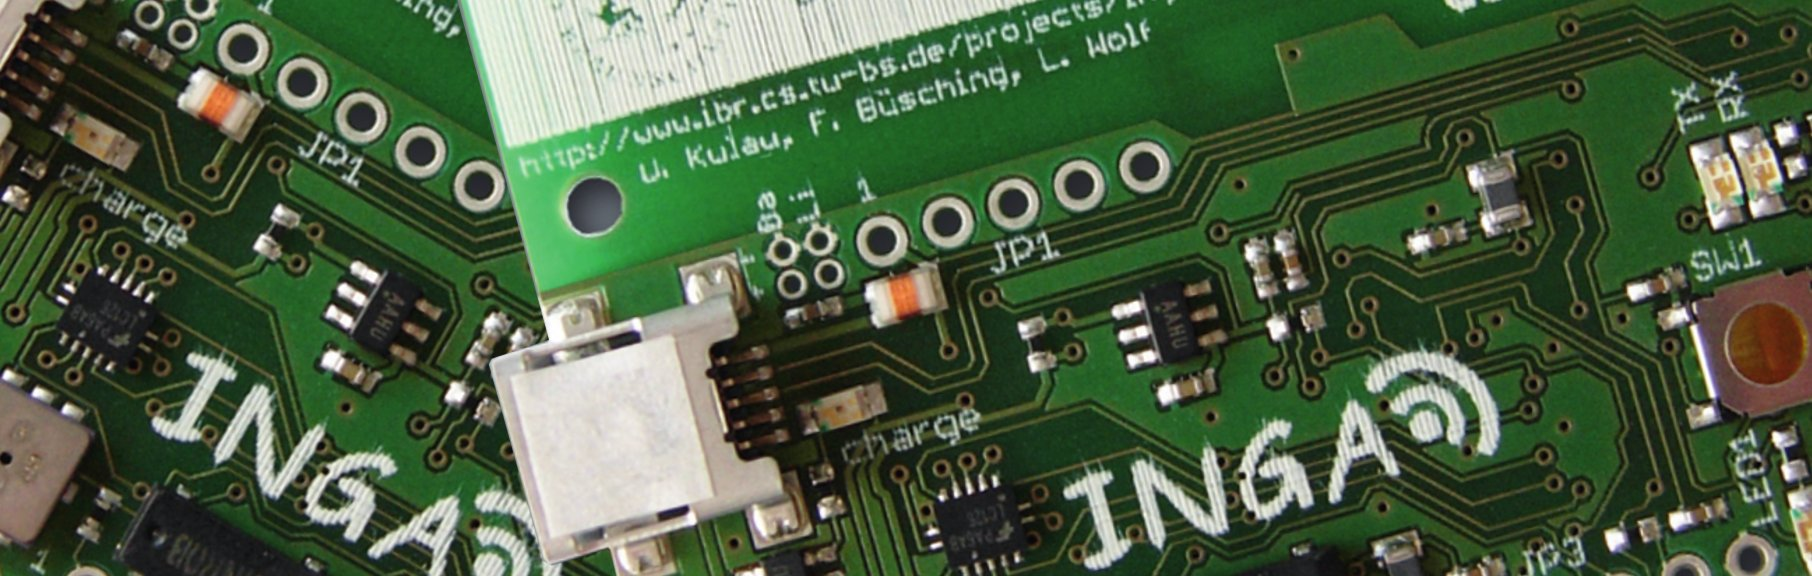
\includegraphics{titlepicture3.jpg}}

% Logo, dass auf Titelseiten oben rechts und auf Inthaltsseiten unten rechts
% dargestellt wird. Es wird jeweils automatisch skliert
\logo{
\includegraphics{ibr.jpg}}
%\logo{Institut für Unkreativität\\und Schreibschwäche}

\begin{document}

\begin{frame}[plain]
\titlepage
\end{frame}

\begin{frame}{Kurze Wiederholung: Idee}
	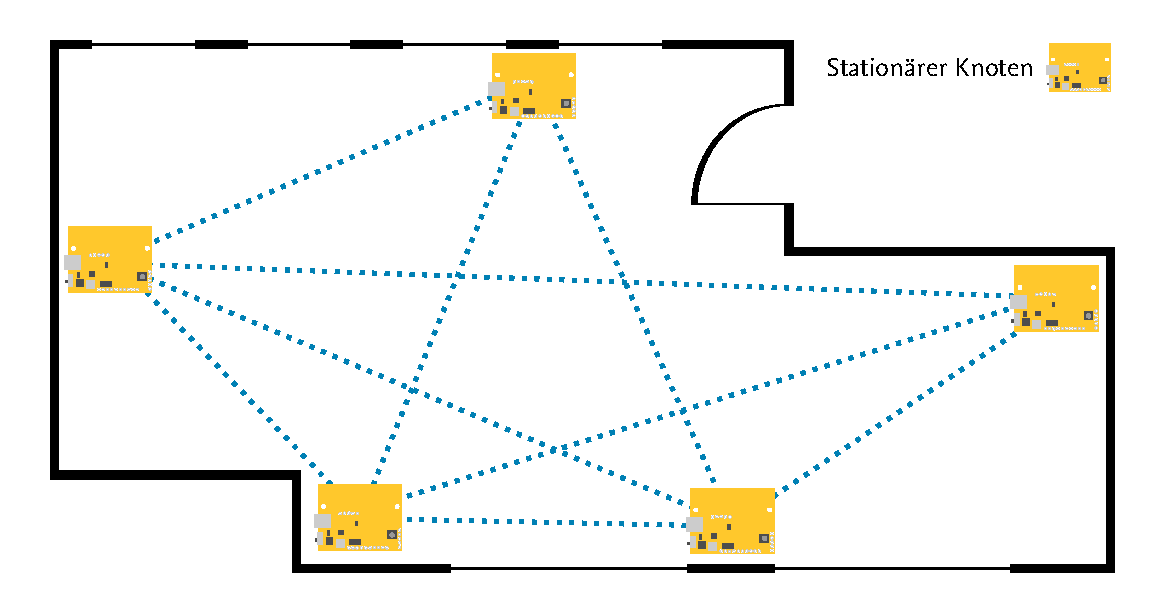
\includegraphics[width=0.48\textwidth]{room-2.pdf}
	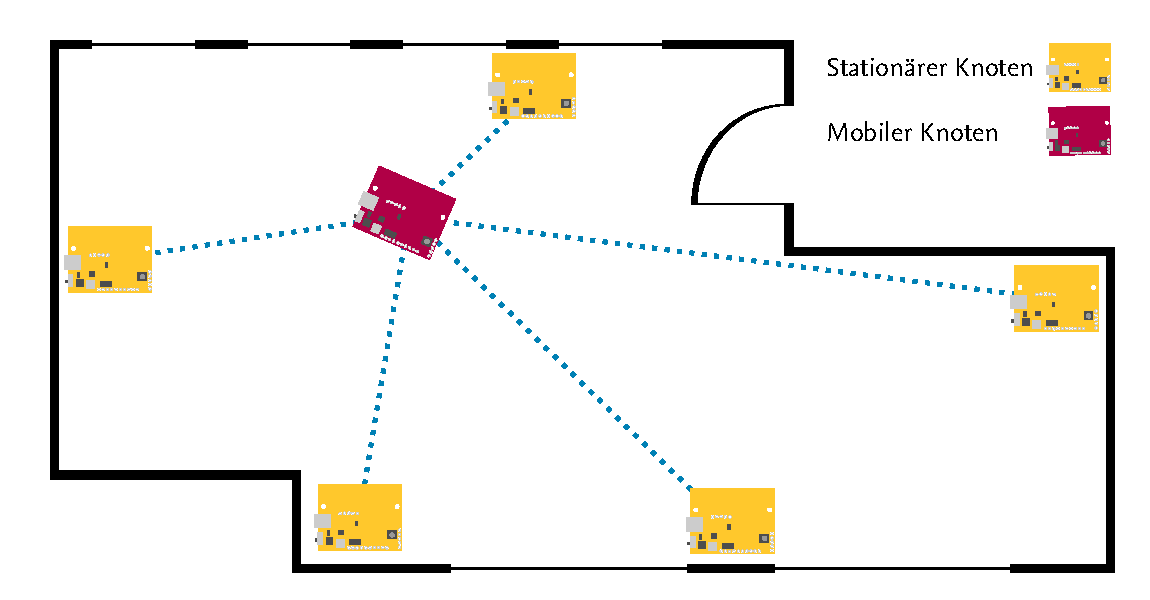
\includegraphics[width=0.48\textwidth]{room-3.pdf}

	\begin{itemize}
		\item Stationäre Knoten bestimmen ihre relative Lage zueinander
		\item Anschließend werden mobile Knoten geortet
		\item Beides geschieht über Laufzeitmessung akustischer Signale
	\end{itemize}
\end{frame}

\begin{frame}{Aktueller Status}
Was geht:
	\begin{itemize}
		\item Test
	\end{itemize}

Was noch nicht geht:
	\begin{itemize}
		\item Test
	\end{itemize}
\end{frame}

\end{document}
